%% ------------------------------------------------------------------------- %%
\chapter{Introdução}
\label{cap:introducao}

Os avanços nos campos tecnológicos e computacionais levaram uma enorme expansão
dos ecossistemas de \textit{software}. Novos programas são criados para
suprir as necessidades dos mais diversos domínios, seja através de sistemas web
codificados em linguagens de \textit{script}; ou por componentes para
sistemas operacionais destinados a embarcados, com a finalidade de controlar algum
recurso do \textit{hardware}. Independente da razão por trás do desenvolvimento
do \textit{software}, é certo que, em alguma etapa, seu código será transformado em linguagem
de máquina por um compilador, mesmo que ele seja executado por um
interpretador.

Um compilador nada mais é que um \textit{software} que traduz um código em uma linguagem
de programação $A$ para outra linguagem $B$ \citep{dragonbook}.  Compiladores
são programas enormes, largamente adotados pela indústria e academia, onde muito
esforço e pesquisa foi e ainda é empregado para que eles produzam código
eficiente, com destaque a corretude. Existem projetos enormes destinados a desenvolvê-los e
aprimorá-los, como o Gnu Compiler Collection
(GCC\footnote{https://gcc.gnu.org/}), capaz de traduzir diversas linguagens
como C, C++ e Fortran, para linguagem de máquina. Há também outros projetos
menores como o F2C\footnote{https://www.netlib.org/f2c/}, um compilador de
Fortran para C, utilizado em ambientes onde não há um compilador Fortran
disponível.

Embora seja possível escrever código em linguagem de máquina, o que
tornaria um compilador desnecessário, isto é extremamente caro e
sujeito a erros, além de ser uma prática extremamente
incomum nos projetos contemporâneos a este trabalho \citep{githuboctoverse} (vide
Figura \ref{fig:github_2017}). Escrever programas em código de máquina tende a
ser trabalhoso e financeiramente custoso, com difícil manutenção e quase impossível portabilidade.
Um exemplo disso é o \textit{Internal Revenue Service} (IRS) dos Estados Unidos,
que ainda mantém máquinas compatíveis com o IBM System/360 devido a existência no sistema
de várias linhas de código escritas em linguagem de montagem para essa
arquitetura \citep{gao}. Esse problema ganhou visibilidade na imprensa após a falha no
\textit{Tax Day} de 2018 \citep{tax_failure}.

%TODO: Deixar essa imagem mais legível
\begin{figure}[ht]
 \centering
 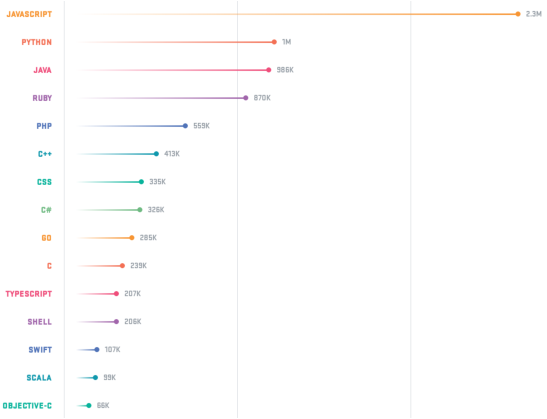
\includegraphics[scale=1.8]{github_2017.pdf}
 \caption{As 15 linguagens mais usadas no GitHub em 2017. Fonte: \cite{githuboctoverse}}
 \label{fig:github_2017}
\end{figure}

Compiladores são usados em projetos dos mais variados tamanhos.
Grandes projetos podem conter milhões de linhas de código, e até mesmo
construir novas linguagens para facilitar o desenvolvimento de novas
funcionalidades. Por exemplo, O GCC contém uma linguagem própria para facilitar
a adição de otimizações na geração de código, que em seguida é
compilado em um único arquivo C, para (1) aproveitar as otimizações já
implementadas no próprio compilador, e (2) evitar reescrever várias
funcionalidades já implementadas. Infelizmente, este processo
gera um gargalo na compilação do projeto em máquinas \textit{manycore}, pois o
GCC não é capaz de compilar um arquivo em paralelo de maneira incremental.

Até então, todo o o
paralelismo na fase de compilação é providenciado ou apenas pelo

Atualmente, todo o paralelismo na fase de compilação é provido pelo GCC de
duas maneiras distintas: ou pelo GNU Make\footnote{https://www.gnu.org/software/make/}, 
que apenas fornece uma granularidade a nível dos arquivos; ou através da estrutura do 
LTO, que será abordada na Seção \ref{chap:related_works}. Esse gargalo pode parecer uma
característica peculiar do projeto GCC, mas discussões com a comunidade levaram
usuários a relatar o mesmo problema em seus projetos. Tal problema pode ser
mitigado por um compilador que seja capaz de compilar um único arquivo em paralelo
\citep{mailgcc} \citep{phoronix}.  Outra possível solução seria 
partir o arquivo em arquivos menores e utilizar o esquema de
paralelismo já existente do GNU Make, mas isto implica em uma modificação na
estrutura do projeto, o que pode não ser o ideal.

Outro caso interessante é a avaliação de expressões constantes. Compiladores
modernos são capazes de avaliar código no qual todos os parâmetros são conhecidos
de antemão, com a finalidade de evitar cálculos em tempo de execução. Essa técnica é
conhecida como \textit{constant folding} \citep{dragonbook} e tornou-se tornou-se
tão comum a ponto de o padrão C++1z adicionar algo
relacionado a isto em sua especificação através do acrônimo \texttt{constexpr}
\citep{iso148822017}.
Sendo assim, talvez o compilador seja capaz de paralelizar esse tipo de
computação, o que implicaria em ganhos para projetos pequenos, com poucos
arquivos.

Considerando que atualmente há uma tendência para que os processadores sejam
cada vez mais paralelos, compiladores que usufruam deste recurso poderiam
reduzir o tempo de compilação de um projeto, ou de uma suíte de testes que
necessita recompilação antes de sua execução, economizando recursos no caso da
computação ser cobrada por hora. Até então, o paralelismo empregado em compiladores
otimizadores foi consequência de uma estrutura criada para permitir otimizações
mais agressivas e custosas, como o LTO \citep{glek2010optimizing}.

Deve ser observado que nem todos os processos de um compilador podem ser
paralelizados. Compiladores operam em etapas que podem ser fortemente
dependentes do resultado da etapa anterior. Por exemplo, ao compilar uma
função em C, pode ser necessário saber se alguma outra foi declarada anteriormente; ou
então o analisador sintático pode alterar um estado do analisador léxico para
detectar variáveis de um novo tipo. Além disto, compiladores também se apoiam em algoritmos
em grafos, cujo paralelismo é um desafio \citep{lumsdaine2007challenges}.

% TODO: Deixar as questões de pesquisa mais detalhadas, e talvez colocar em outra
% subseção.
Sendo assim, existe interesse em pesquisas que apontem onde exatamente um compilador
pode tirar vantagem de paralelismo, e esta é a questão de pesquisa que este
trabalho aborda. Portanto, esse trabalho propõe uma alternativa ao LTO com foco
em desenvolvimento incremental, cobrindo os casos onde o LTO produz binários menos
eficientes através de melhorias no paralelismo do processo clássico de compilação.
Para validar os resultados, este trabalho inclui a implementação no GCC de algumas das
técnicas discutidas, além da utilização de técnicas de inferência estatística para
análises no tempo total de compilação no projeto GCC e arquivos separados.
